\chapter{Understanding Heat Exchanger}
\begin{docspec}
	"Of course, they are not directly called heat exchangers in our daily life. They can be found in many devices around us: computers, refrigerators, radiators, mobiles phones and etc. I promise many of us live with them every day. Just imagine a hot summer day, you have to sit a room without an air conditioner or have a warm coke if you don't have a fridge."----\textbf{A comment from Dr.Qian}
\end{docspec}
Unlike previous notes, in Lab5 we will focus on indicators of heat exchange efficiency and make quantitative comparison of various heat exchangers, i.e., engineering side of things. At the end, we will also discuss elementary design principles of heat exchanger.

\section{Basic Working Principles of Heat Exchanger}
Heat exchanger, by definition, is any device that exchange heat between two or more fluids\footnote{Heat exchanger can also transfer heat between gas and liquid, a multiphase process.} of different temperatures.  The basic components of heat exchangers include: (1) flow path of cold fluid, (2) flow path of hot fluid, and (3) a separator\index{separator} to prevent direct contact between the cold and the hot\footnote{some heat exchangers might allow direct mixing between two distinct fluids, so fluids are not totally separated in those exchangers}.

Regardless of the design, the underlying principles that heat exchangers work upon are laws of thermodynamics\footnote{Even though they are called the "laws", thermodynamics is actually an empirical subject, i.e., these laws are summarized solely based upon experimental results, and are not, at least for now, logically derivable.}. While the zeroth law of thermodynamics\index{zeroth law of thermodynamics} demands us to \imp{create temperature difference to simply make energy flow happen}, the first and second laws of thermodynamics are the guidelines for engineers to fine-tune the energy flow in heat exchangers to improve the energy efficiency while keep the operating cost modest.  

The first law of thermodynamics\index{first law of thermodynamics} dictates how we construct governing equation for describing energy flow in the exchangers. Because the energy cannot be destroyed or created, any amount of energy goes into the heat exchanger will cause equal amount of decrease in energy in its surrounding environment. The governing equation is then established upon the conservation of energy, and has terms for what is happening inside heat exchanger at one side and has terms related to environmental changes the other side, i.e.,
\begin{equation}
	\Delta U_{exchanger} = -\Delta U_{environment}.
\end{equation}

The second law of thermodynamics\index{second law of thermodynamics} sheds light on the way of how we are supposed to delay or accelerate the process of exchangers achieving their thermal equilibrium. A thermal equilibrium is achieved when the entropy\footnote{the entropy is defined as the ratio of change in heat over temperature, i.e., $\Delta S = \frac{\Delta Q}{T}$} of the system is maximized. According to the second law, the only changes possible at an equilibrium state are the ones that further increase system entropy.
\section{Common Types of Heat Exchangers}
Heat exchangers fall into different classes based on their \imp{flow configuration, construction method, and heat transfer mechanism}. Commonly used flow configurations are: concurrent flow, countercurrent flow, cross flow, and hybrid flow. The schematic of how the distinct fluid streams flow in these configurations are shown in Fig. \ref{fig:flowschematic} and \ref{fig:flowschematic2}, where no direct mixing is allowed in all the configurations.
\begin{figure*}
	% Gradient Info
	\tikzset {_pi9b0e0z4/.code = {\pgfsetadditionalshadetransform{ \pgftransformshift{\pgfpoint{0 bp } { 0 bp }  }  \pgftransformrotate{0 }  \pgftransformscale{2 }  }}}
	\pgfdeclarehorizontalshading{_zca4czzo0}{150bp}{rgb(0bp)=(0.99,0.13,0.13);
		rgb(37.5bp)=(0.99,0.13,0.13);
		rgb(60.6547600882394bp)=(0.98,0.35,0.35);
		rgb(100bp)=(0.98,0.35,0.35)}
	
	% Gradient Info
	
	\tikzset {_daeh4bqqw/.code = {\pgfsetadditionalshadetransform{ \pgftransformshift{\pgfpoint{0 bp } { 0 bp }  }  \pgftransformrotate{0 }  \pgftransformscale{2 }  }}}
	\pgfdeclarehorizontalshading{_fd12v17u7}{150bp}{rgb(0bp)=(0.99,0.24,0.24);
		rgb(37.5bp)=(0.99,0.24,0.24);
		rgb(53.33928516932896bp)=(1,0.68,0.68);
		rgb(62.5bp)=(1,0.68,0.68);
		rgb(100bp)=(1,0.68,0.68)}
	
	% Gradient Info
	
	\tikzset {_1t0u11t9h/.code = {\pgfsetadditionalshadetransform{ \pgftransformshift{\pgfpoint{0 bp } { 0 bp }  }  \pgftransformrotate{0 }  \pgftransformscale{2 }  }}}
	\pgfdeclarehorizontalshading{_4t2izn1sy}{150bp}{rgb(0bp)=(0.99,0.13,0.13);
		rgb(37.5bp)=(0.99,0.13,0.13);
		rgb(60.6547600882394bp)=(0.98,0.35,0.35);
		rgb(100bp)=(0.98,0.35,0.35)}
	
	% Gradient Info
	\tikzset {_4q3t9tmzv/.code = {\pgfsetadditionalshadetransform{ \pgftransformshift{\pgfpoint{0 bp } { 0 bp }  }  \pgftransformrotate{0 }  \pgftransformscale{2 }  }}}
	\pgfdeclarehorizontalshading{_5r932h84a}{150bp}{rgb(0bp)=(0.99,0.24,0.24);
		rgb(37.5bp)=(0.99,0.24,0.24);
		rgb(53.33928516932896bp)=(1,0.68,0.68);
		rgb(62.5bp)=(1,0.68,0.68);
		rgb(100bp)=(1,0.68,0.68)}
	\tikzset{every picture/.style={line width=0.75pt}} %set default line width to 0.75pt        
	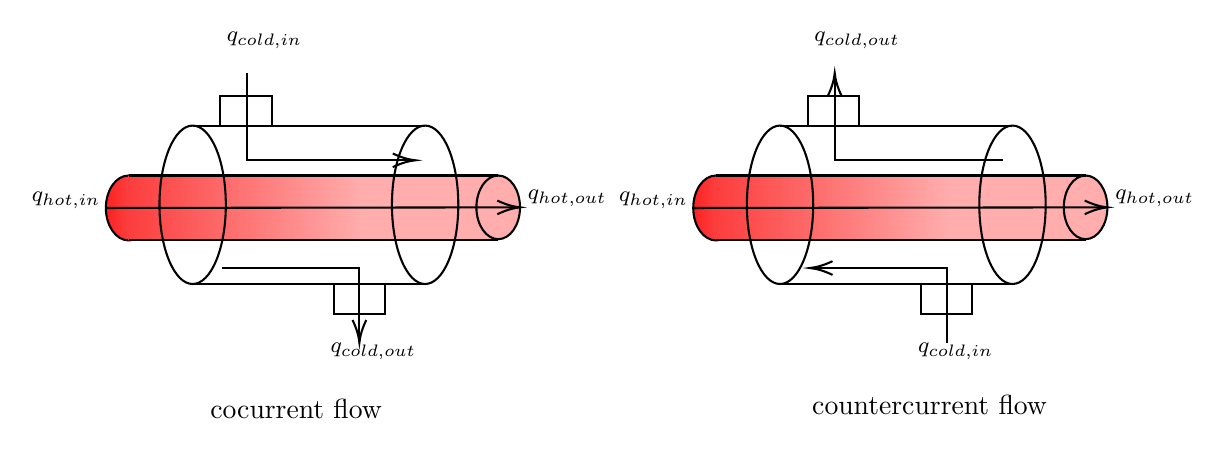
\begin{tikzpicture}[x=0.75pt,y=0.75pt,yscale=-1,xscale=1]
		%uncomment if require: \path (0,300); %set diagram left start at 0, and has height of 300
		
		%Shape: Ellipse [id:dp5569940089135211] 
		\path  [shading=_zca4czzo0,_pi9b0e0z4] (85.17,104.37) .. controls (85.17,95.73) and (90.07,88.73) .. (96.13,88.73) .. controls (102.18,88.73) and (107.09,95.73) .. (107.09,104.37) .. controls (107.09,113) and (102.18,120) .. (96.13,120) .. controls (90.07,120) and (85.17,113) .. (85.17,104.37) -- cycle ; % for fading 
		\draw  [color={rgb, 255:red, 0; green, 0; blue, 0 }  ,draw opacity=1 ] (85.17,104.37) .. controls (85.17,95.73) and (90.07,88.73) .. (96.13,88.73) .. controls (102.18,88.73) and (107.09,95.73) .. (107.09,104.37) .. controls (107.09,113) and (102.18,120) .. (96.13,120) .. controls (90.07,120) and (85.17,113) .. (85.17,104.37) -- cycle ; % for border 
		
		%Flowchart: Process [id:dp6758619041277437] 
		\draw  [draw opacity=0][shading=_fd12v17u7,_daeh4bqqw][line width=0.75]  (96.13,88.73) -- (274.2,88.73) -- (274.2,120) -- (96.13,120) -- cycle ;
		%Shape: Ellipse [id:dp6104734076932498] 
		\draw  [color={rgb, 255:red, 0; green, 0; blue, 0 }  ,draw opacity=1 ] (111,102.83) .. controls (111,81.75) and (118.16,64.67) .. (126.98,64.67) .. controls (135.81,64.67) and (142.97,81.75) .. (142.97,102.83) .. controls (142.97,123.91) and (135.81,141) .. (126.98,141) .. controls (118.16,141) and (111,123.91) .. (111,102.83) -- cycle ;
		%Shape: Ellipse [id:dp4304854978271885] 
		\draw  [color={rgb, 255:red, 0; green, 0; blue, 0 }  ,draw opacity=1 ] (223,102.83) .. controls (223,81.75) and (230.16,64.67) .. (238.98,64.67) .. controls (247.81,64.67) and (254.97,81.75) .. (254.97,102.83) .. controls (254.97,123.91) and (247.81,141) .. (238.98,141) .. controls (230.16,141) and (223,123.91) .. (223,102.83) -- cycle ;
		%Shape: Ellipse [id:dp3968988409962665] 
		\draw  [color={rgb, 255:red, 0; green, 0; blue, 0 }  ,draw opacity=1 ][fill={rgb, 255:red, 255; green, 173; blue, 173 }  ,fill opacity=1 ] (263.7,104.07) .. controls (263.7,95.6) and (268.41,88.73) .. (274.2,88.73) .. controls (280,88.73) and (284.7,95.6) .. (284.7,104.07) .. controls (284.7,112.54) and (280,119.4) .. (274.2,119.4) .. controls (268.41,119.4) and (263.7,112.54) .. (263.7,104.07) -- cycle ;
		%Straight Lines [id:da508132551052004] 
		\draw    (126.98,64.67) -- (238.98,64.67) ;
		%Straight Lines [id:da6260528662795266] 
		\draw    (126.98,141) -- (238.98,141) ;
		%Straight Lines [id:da7713495508657232] 
		\draw    (96.13,88.73) -- (274.2,88.73) ;
		%Straight Lines [id:da33911495236994826] 
		\draw    (96.13,120) -- (274.2,120) ;
		%Shape: Rectangle [id:dp2120589097132366] 
		\draw   (140.33,50.4) -- (165,50.4) -- (165,65) -- (140.33,65) -- cycle ;
		%Shape: Rectangle [id:dp42642209601906944] 
		\draw   (194.98,141) -- (219.65,141) -- (219.65,155.6) -- (194.98,155.6) -- cycle ;
		%Straight Lines [id:da3665468056013994] 
		\draw    (85.17,104.37) -- (282.7,104.07) ;
		\draw [shift={(284.7,104.07)}, rotate = 539.9100000000001] [color={rgb, 255:red, 0; green, 0; blue, 0 }  ][line width=0.75]    (10.93,-3.29) .. controls (6.95,-1.4) and (3.31,-0.3) .. (0,0) .. controls (3.31,0.3) and (6.95,1.4) .. (10.93,3.29)   ;
		%Straight Lines [id:da8151931788039299] 
		\draw    (153.33,39.4) -- (153.33,81.4) -- (232.33,81.4) ;
		\draw [shift={(234.33,81.4)}, rotate = 180] [color={rgb, 255:red, 0; green, 0; blue, 0 }  ][line width=0.75]    (10.93,-3.29) .. controls (6.95,-1.4) and (3.31,-0.3) .. (0,0) .. controls (3.31,0.3) and (6.95,1.4) .. (10.93,3.29)   ;
		%Straight Lines [id:da9967303831292222] 
		\draw    (141.33,133.3) -- (207.32,133.3) -- (207.32,167.3) ;
		\draw [shift={(207.32,169.3)}, rotate = 270] [color={rgb, 255:red, 0; green, 0; blue, 0 }  ][line width=0.75]    (10.93,-3.29) .. controls (6.95,-1.4) and (3.31,-0.3) .. (0,0) .. controls (3.31,0.3) and (6.95,1.4) .. (10.93,3.29)   ;
		%Shape: Ellipse [id:dp7125812606209282] 
		\path  [shading=_4t2izn1sy,_1t0u11t9h] (368.17,104.37) .. controls (368.17,95.73) and (373.07,88.73) .. (379.13,88.73) .. controls (385.18,88.73) and (390.09,95.73) .. (390.09,104.37) .. controls (390.09,113) and (385.18,120) .. (379.13,120) .. controls (373.07,120) and (368.17,113) .. (368.17,104.37) -- cycle ; % for fading 
		\draw  [color={rgb, 255:red, 0; green, 0; blue, 0 }  ,draw opacity=1 ] (368.17,104.37) .. controls (368.17,95.73) and (373.07,88.73) .. (379.13,88.73) .. controls (385.18,88.73) and (390.09,95.73) .. (390.09,104.37) .. controls (390.09,113) and (385.18,120) .. (379.13,120) .. controls (373.07,120) and (368.17,113) .. (368.17,104.37) -- cycle ; % for border 
		
		%Flowchart: Process [id:dp9386334262995394] 
		\draw  [draw opacity=0][shading=_5r932h84a,_4q3t9tmzv][line width=0.75]  (379.13,88.73) -- (557.2,88.73) -- (557.2,120) -- (379.13,120) -- cycle ;
		%Shape: Ellipse [id:dp08547853477676937] 
		\draw  [color={rgb, 255:red, 0; green, 0; blue, 0 }  ,draw opacity=1 ] (394,102.83) .. controls (394,81.75) and (401.16,64.67) .. (409.98,64.67) .. controls (418.81,64.67) and (425.97,81.75) .. (425.97,102.83) .. controls (425.97,123.91) and (418.81,141) .. (409.98,141) .. controls (401.16,141) and (394,123.91) .. (394,102.83) -- cycle ;
		%Shape: Ellipse [id:dp5096570584699526] 
		\draw  [color={rgb, 255:red, 0; green, 0; blue, 0 }  ,draw opacity=1 ] (506,102.83) .. controls (506,81.75) and (513.16,64.67) .. (521.98,64.67) .. controls (530.81,64.67) and (537.97,81.75) .. (537.97,102.83) .. controls (537.97,123.91) and (530.81,141) .. (521.98,141) .. controls (513.16,141) and (506,123.91) .. (506,102.83) -- cycle ;
		%Shape: Ellipse [id:dp833314682214128] 
		\draw  [color={rgb, 255:red, 0; green, 0; blue, 0 }  ,draw opacity=1 ][fill={rgb, 255:red, 255; green, 173; blue, 173 }  ,fill opacity=1 ] (546.7,104.07) .. controls (546.7,95.6) and (551.41,88.73) .. (557.2,88.73) .. controls (563,88.73) and (567.7,95.6) .. (567.7,104.07) .. controls (567.7,112.54) and (563,119.4) .. (557.2,119.4) .. controls (551.41,119.4) and (546.7,112.54) .. (546.7,104.07) -- cycle ;
		%Straight Lines [id:da5579124681472262] 
		\draw    (409.98,64.67) -- (521.98,64.67) ;
		%Straight Lines [id:da3860769654716606] 
		\draw    (409.98,141) -- (521.98,141) ;
		%Straight Lines [id:da8168098552830327] 
		\draw    (379.13,88.73) -- (557.2,88.73) ;
		%Straight Lines [id:da25673877656483735] 
		\draw    (379.13,120) -- (557.2,120) ;
		%Shape: Rectangle [id:dp7480093930577298] 
		\draw   (423.33,50.4) -- (448,50.4) -- (448,65) -- (423.33,65) -- cycle ;
		%Shape: Rectangle [id:dp03787723134370358] 
		\draw   (477.98,141) -- (502.65,141) -- (502.65,155.6) -- (477.98,155.6) -- cycle ;
		%Straight Lines [id:da8399591824551974] 
		\draw    (368.17,104.37) -- (565.7,104.07) ;
		\draw [shift={(567.7,104.07)}, rotate = 539.9100000000001] [color={rgb, 255:red, 0; green, 0; blue, 0 }  ][line width=0.75]    (10.93,-3.29) .. controls (6.95,-1.4) and (3.31,-0.3) .. (0,0) .. controls (3.31,0.3) and (6.95,1.4) .. (10.93,3.29)   ;
		%Straight Lines [id:da5467424763409797] 
		\draw    (436.33,41.4) -- (436.33,81.4) -- (517.33,81.4) ;
		\draw [shift={(436.33,39.4)}, rotate = 90] [color={rgb, 255:red, 0; green, 0; blue, 0 }  ][line width=0.75]    (10.93,-3.29) .. controls (6.95,-1.4) and (3.31,-0.3) .. (0,0) .. controls (3.31,0.3) and (6.95,1.4) .. (10.93,3.29)   ;
		%Straight Lines [id:da2825617904620995] 
		\draw    (426.33,133.3) -- (490.32,133.3) -- (490.32,169.3) ;
		\draw [shift={(424.33,133.3)}, rotate = 0] [color={rgb, 255:red, 0; green, 0; blue, 0 }  ][line width=0.75]    (10.93,-3.29) .. controls (6.95,-1.4) and (3.31,-0.3) .. (0,0) .. controls (3.31,0.3) and (6.95,1.4) .. (10.93,3.29)   ;
		
		% Text Node
		\draw (48,95) node [anchor=north west][inner sep=0.75pt]  [font=\footnotesize]  {$q_{hot,in}$};
		% Text Node
		\draw (287,94) node [anchor=north west][inner sep=0.75pt]  [font=\footnotesize]  {$q_{hot,out}$};
		% Text Node
		\draw (142,18) node [anchor=north west][inner sep=0.75pt]  [font=\footnotesize]  {$q_{cold,in}$};
		% Text Node
		\draw (192,168) node [anchor=north west][inner sep=0.75pt]  [font=\footnotesize]  {$q_{cold,out}$};
		% Text Node
		\draw (331,95) node [anchor=north west][inner sep=0.75pt]  [font=\footnotesize]  {$q_{hot,in}$};
		% Text Node
		\draw (570,94) node [anchor=north west][inner sep=0.75pt]  [font=\footnotesize]  {$q_{hot,out}$};
		% Text Node
		\draw (425,18) node [anchor=north west][inner sep=0.75pt]  [font=\footnotesize]  {$q_{cold,out}$};
		% Text Node
		\draw (475,168) node [anchor=north west][inner sep=0.75pt]  [font=\footnotesize]  {$q_{cold,in}$};
		% Text Node
		\draw (134,195) node [anchor=north west][inner sep=0.75pt]   [align=left] {cocurrent flow};
		% Text Node
		\draw (424,193) node [anchor=north west][inner sep=0.75pt]   [align=left] {countercurrent flow};
		
		
	\end{tikzpicture}
	\caption{Cocurrent and countercurrent flow configurations in heat exchangers}
	\label{fig:flowschematic}
\end{figure*}
\begin{figure*}
% Gradient Info
\tikzset {_kashen0mv/.code = {\pgfsetadditionalshadetransform{ \pgftransformshift{\pgfpoint{0 bp } { 0 bp }  }  \pgftransformrotate{0 }  \pgftransformscale{2 }  }}}
\pgfdeclarehorizontalshading{_19ahpion0}{150bp}{rgb(0bp)=(0.99,0.13,0.13);
	rgb(37.5bp)=(0.99,0.13,0.13);
	rgb(60.6547600882394bp)=(0.98,0.35,0.35);
	rgb(100bp)=(0.98,0.35,0.35)}

% Gradient Info

\tikzset {_j9sjuh7ca/.code = {\pgfsetadditionalshadetransform{ \pgftransformshift{\pgfpoint{0 bp } { 0 bp }  }  \pgftransformrotate{0 }  \pgftransformscale{2 }  }}}
\pgfdeclarehorizontalshading{_1b823t7mb}{150bp}{rgb(0bp)=(0.99,0.24,0.24);
	rgb(37.5bp)=(0.99,0.24,0.24);
	rgb(53.33928516932896bp)=(1,0.68,0.68);
	rgb(62.5bp)=(1,0.68,0.68);
	rgb(100bp)=(1,0.68,0.68)}

% Gradient Info

\tikzset {_wc7ixlhve/.code = {\pgfsetadditionalshadetransform{ \pgftransformshift{\pgfpoint{0 bp } { 0 bp }  }  \pgftransformrotate{0 }  \pgftransformscale{2 }  }}}
\pgfdeclarehorizontalshading{_zmj4d84wq}{150bp}{rgb(0bp)=(0.99,0.13,0.13);
	rgb(37.5bp)=(0.99,0.13,0.13);
	rgb(60.6547600882394bp)=(0.98,0.35,0.35);
	rgb(100bp)=(0.98,0.35,0.35)}

% Gradient Info

\tikzset {_7qylw7422/.code = {\pgfsetadditionalshadetransform{ \pgftransformshift{\pgfpoint{0 bp } { 0 bp }  }  \pgftransformrotate{0 }  \pgftransformscale{2 }  }}}
\pgfdeclarehorizontalshading{_ifd39xq06}{150bp}{rgb(0bp)=(0.99,0.24,0.24);
	rgb(37.5bp)=(0.99,0.24,0.24);
	rgb(53.33928516932896bp)=(1,0.68,0.68);
	rgb(62.5bp)=(1,0.68,0.68);
	rgb(100bp)=(1,0.68,0.68)}
\tikzset{every picture/.style={line width=0.75pt}} %set default line width to 0.75pt        

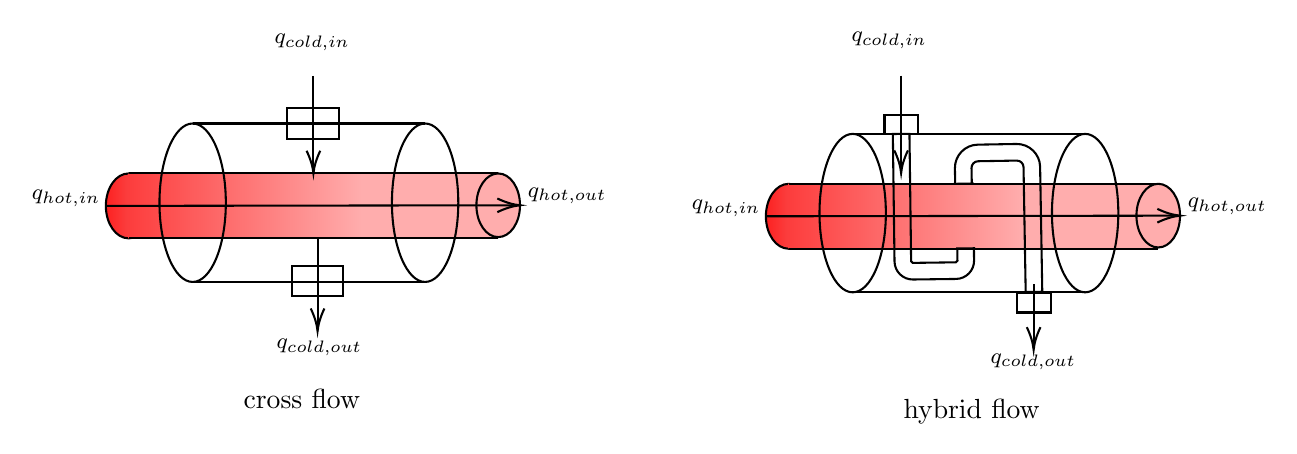
\begin{tikzpicture}[x=0.75pt,y=0.75pt,yscale=-1,xscale=1]
	%uncomment if require: \path (0,300); %set diagram left start at 0, and has height of 300
	%Shape: Ellipse [id:dp79651783665876] 
	\path  [shading=_19ahpion0,_kashen0mv] (54.17,125.37) .. controls (54.17,116.73) and (59.07,109.73) .. (65.13,109.73) .. controls (71.18,109.73) and (76.09,116.73) .. (76.09,125.37) .. controls (76.09,134) and (71.18,141) .. (65.13,141) .. controls (59.07,141) and (54.17,134) .. (54.17,125.37) -- cycle ; % for fading 
	\draw  [color={rgb, 255:red, 0; green, 0; blue, 0 }  ,draw opacity=1 ] (54.17,125.37) .. controls (54.17,116.73) and (59.07,109.73) .. (65.13,109.73) .. controls (71.18,109.73) and (76.09,116.73) .. (76.09,125.37) .. controls (76.09,134) and (71.18,141) .. (65.13,141) .. controls (59.07,141) and (54.17,134) .. (54.17,125.37) -- cycle ; % for border 
	
	%Flowchart: Process [id:dp08903171521051856] 
	\draw  [draw opacity=0][shading=_1b823t7mb,_j9sjuh7ca][line width=0.75]  (65.13,109.73) -- (243.2,109.73) -- (243.2,141) -- (65.13,141) -- cycle ;
	%Shape: Ellipse [id:dp5696641954355333] 
	\draw  [color={rgb, 255:red, 0; green, 0; blue, 0 }  ,draw opacity=1 ] (80,123.83) .. controls (80,102.75) and (87.16,85.67) .. (95.98,85.67) .. controls (104.81,85.67) and (111.97,102.75) .. (111.97,123.83) .. controls (111.97,144.91) and (104.81,162) .. (95.98,162) .. controls (87.16,162) and (80,144.91) .. (80,123.83) -- cycle ;
	%Shape: Ellipse [id:dp5086024981750389] 
	\draw  [color={rgb, 255:red, 0; green, 0; blue, 0 }  ,draw opacity=1 ] (192,123.83) .. controls (192,102.75) and (199.16,85.67) .. (207.98,85.67) .. controls (216.81,85.67) and (223.97,102.75) .. (223.97,123.83) .. controls (223.97,144.91) and (216.81,162) .. (207.98,162) .. controls (199.16,162) and (192,144.91) .. (192,123.83) -- cycle ;
	%Shape: Ellipse [id:dp5561774227003878] 
	\draw  [color={rgb, 255:red, 0; green, 0; blue, 0 }  ,draw opacity=1 ][fill={rgb, 255:red, 255; green, 173; blue, 173 }  ,fill opacity=1 ] (232.7,125.07) .. controls (232.7,116.6) and (237.41,109.73) .. (243.2,109.73) .. controls (249,109.73) and (253.7,116.6) .. (253.7,125.07) .. controls (253.7,133.54) and (249,140.4) .. (243.2,140.4) .. controls (237.41,140.4) and (232.7,133.54) .. (232.7,125.07) -- cycle ;
	%Straight Lines [id:da9347132497675555] 
	\draw    (95.98,85.67) -- (207.98,85.67) ;
	%Straight Lines [id:da9970261608535496] 
	\draw    (95.98,162) -- (207.98,162) ;
	%Straight Lines [id:da006308564767346869] 
	\draw    (65.13,109.73) -- (243.2,109.73) ;
	%Straight Lines [id:da3801899638500196] 
	\draw    (65.13,141) -- (243.2,141) ;
	%Shape: Rectangle [id:dp5724762544379602] 
	\draw   (141.65,78.37) -- (166.32,78.37) -- (166.32,92.97) -- (141.65,92.97) -- cycle ;
	%Straight Lines [id:da08280314221076734] 
	\draw    (54.17,125.37) -- (251.7,125.07) ;
	\draw [shift={(253.7,125.07)}, rotate = 539.9100000000001] [color={rgb, 255:red, 0; green, 0; blue, 0 }  ][line width=0.75]    (10.93,-3.29) .. controls (6.95,-1.4) and (3.31,-0.3) .. (0,0) .. controls (3.31,0.3) and (6.95,1.4) .. (10.93,3.29)   ;
	%Straight Lines [id:da7658121151799667] 
	\draw    (154.17,62.73) -- (154.17,107.73) ;
	\draw [shift={(154.17,109.73)}, rotate = 270] [color={rgb, 255:red, 0; green, 0; blue, 0 }  ][line width=0.75]    (10.93,-3.29) .. controls (6.95,-1.4) and (3.31,-0.3) .. (0,0) .. controls (3.31,0.3) and (6.95,1.4) .. (10.93,3.29)   ;
	%Shape: Rectangle [id:dp09996446981925655] 
	\draw   (143.65,154.37) -- (168.32,154.37) -- (168.32,168.97) -- (143.65,168.97) -- cycle ;
	%Straight Lines [id:da5556278608545433] 
	\draw    (156.17,141) -- (156.17,183.73) ;
	\draw [shift={(156.17,185.73)}, rotate = 270] [color={rgb, 255:red, 0; green, 0; blue, 0 }  ][line width=0.75]    (10.93,-3.29) .. controls (6.95,-1.4) and (3.31,-0.3) .. (0,0) .. controls (3.31,0.3) and (6.95,1.4) .. (10.93,3.29)   ;
	%Shape: Ellipse [id:dp2695433445813036] 
	\path  [shading=_zmj4d84wq,_wc7ixlhve] (372.17,130.37) .. controls (372.17,121.73) and (377.07,114.73) .. (383.13,114.73) .. controls (389.18,114.73) and (394.09,121.73) .. (394.09,130.37) .. controls (394.09,139) and (389.18,146) .. (383.13,146) .. controls (377.07,146) and (372.17,139) .. (372.17,130.37) -- cycle ; % for fading 
	\draw  [color={rgb, 255:red, 0; green, 0; blue, 0 }  ,draw opacity=1 ] (372.17,130.37) .. controls (372.17,121.73) and (377.07,114.73) .. (383.13,114.73) .. controls (389.18,114.73) and (394.09,121.73) .. (394.09,130.37) .. controls (394.09,139) and (389.18,146) .. (383.13,146) .. controls (377.07,146) and (372.17,139) .. (372.17,130.37) -- cycle ; % for border 
	
	%Flowchart: Process [id:dp9926349168278463] 
	\draw  [draw opacity=0][shading=_ifd39xq06,_7qylw7422][line width=0.75]  (383.13,114.73) -- (561.2,114.73) -- (561.2,146) -- (383.13,146) -- cycle ;
	%Shape: Ellipse [id:dp27046713277779] 
	\draw  [color={rgb, 255:red, 0; green, 0; blue, 0 }  ,draw opacity=1 ] (398,128.83) .. controls (398,107.75) and (405.16,90.67) .. (413.98,90.67) .. controls (422.81,90.67) and (429.97,107.75) .. (429.97,128.83) .. controls (429.97,149.91) and (422.81,167) .. (413.98,167) .. controls (405.16,167) and (398,149.91) .. (398,128.83) -- cycle ;
	%Shape: Ellipse [id:dp5720750183843122] 
	\draw  [color={rgb, 255:red, 0; green, 0; blue, 0 }  ,draw opacity=1 ] (510,128.83) .. controls (510,107.75) and (517.16,90.67) .. (525.98,90.67) .. controls (534.81,90.67) and (541.97,107.75) .. (541.97,128.83) .. controls (541.97,149.91) and (534.81,167) .. (525.98,167) .. controls (517.16,167) and (510,149.91) .. (510,128.83) -- cycle ;
	%Shape: Ellipse [id:dp5475334767054657] 
	\draw  [color={rgb, 255:red, 0; green, 0; blue, 0 }  ,draw opacity=1 ][fill={rgb, 255:red, 255; green, 173; blue, 173 }  ,fill opacity=1 ] (550.7,130.07) .. controls (550.7,121.6) and (555.41,114.73) .. (561.2,114.73) .. controls (567,114.73) and (571.7,121.6) .. (571.7,130.07) .. controls (571.7,138.54) and (567,145.4) .. (561.2,145.4) .. controls (555.41,145.4) and (550.7,138.54) .. (550.7,130.07) -- cycle ;
	%Straight Lines [id:da03670575640467655] 
	\draw    (413.98,90.67) -- (525.98,90.67) ;
	%Straight Lines [id:da9045161505185109] 
	\draw    (413.98,167) -- (525.98,167) ;
	%Straight Lines [id:da036461917848550685] 
	\draw    (383.13,114.73) -- (561.2,114.73) ;
	%Straight Lines [id:da7259053840622636] 
	\draw    (383.13,146) -- (561.2,146) ;
	%Straight Lines [id:da9751047575002026] 
	\draw    (372.17,130.37) -- (569.7,130.07) ;
	\draw [shift={(571.7,130.07)}, rotate = 539.9100000000001] [color={rgb, 255:red, 0; green, 0; blue, 0 }  ][line width=0.75]    (10.93,-3.29) .. controls (6.95,-1.4) and (3.31,-0.3) .. (0,0) .. controls (3.31,0.3) and (6.95,1.4) .. (10.93,3.29)   ;
	%Straight Lines [id:da8507154884340133] 
	\draw    (437.32,62.55) -- (437.32,107.55) ;
	\draw [shift={(437.32,109.55)}, rotate = 270] [color={rgb, 255:red, 0; green, 0; blue, 0 }  ][line width=0.75]    (10.93,-3.29) .. controls (6.95,-1.4) and (3.31,-0.3) .. (0,0) .. controls (3.31,0.3) and (6.95,1.4) .. (10.93,3.29)   ;
	%Shape: Rectangle [id:dp4404696825800831] 
	\draw   (493.33,167.37) -- (509.32,167.37) -- (509.32,176.73) -- (493.33,176.73) -- cycle ;
	%Straight Lines [id:da8362094849944305] 
	\draw    (501.17,163) -- (501.17,192.73) ;
	\draw [shift={(501.17,194.73)}, rotate = 270] [color={rgb, 255:red, 0; green, 0; blue, 0 }  ][line width=0.75]    (10.93,-3.29) .. controls (6.95,-1.4) and (3.31,-0.3) .. (0,0) .. controls (3.31,0.3) and (6.95,1.4) .. (10.93,3.29)   ;
	%Shape: Rectangle [id:dp12209234527146329] 
	\draw   (429.33,81.37) -- (445.32,81.37) -- (445.32,90.73) -- (429.33,90.73) -- cycle ;
	%U Turn Arrow [id:dp8989606374525857] 
	\draw   (433.33,90.73) -- (434.14,152.15) .. controls (434.2,157.01) and (438.19,160.89) .. (443.05,160.83) -- (463.79,160.56) .. controls (468.65,160.49) and (472.54,156.5) .. (472.47,151.65) -- (472.4,145.78) -- (472.94,145.78) -- (468.39,145.84) -- (463.85,145.9) -- (464.39,145.89) -- (464.47,151.75) .. controls (464.47,152.19) and (464.13,152.55) .. (463.69,152.55) -- (442.94,152.82) .. controls (442.51,152.83) and (442.15,152.48) .. (442.14,152.04) -- (441.34,90.63) -- cycle ;
	%U Turn Arrow [id:dp738995424326948] 
	\draw   (505.33,166.73) -- (504.29,106.55) .. controls (504.19,100.36) and (499.08,95.43) .. (492.89,95.53) -- (474.26,95.86) .. controls (468.07,95.96) and (463.14,101.07) .. (463.24,107.26) -- (463.37,114.73) -- (462.46,114.75) -- (467.37,114.66) -- (472.28,114.58) -- (471.37,114.59) -- (471.24,107.12) .. controls (471.21,105.35) and (472.62,103.88) .. (474.4,103.85) -- (493.03,103.53) .. controls (494.8,103.5) and (496.27,104.91) .. (496.3,106.69) -- (497.34,166.87) -- cycle ;
	
	% Text Node
	\draw (17,116) node [anchor=north west][inner sep=0.75pt]  [font=\footnotesize]  {$q_{hot,in}$};
	% Text Node
	\draw (256,115) node [anchor=north west][inner sep=0.75pt]  [font=\footnotesize]  {$q_{hot,out}$};
	% Text Node
	\draw (134,41) node [anchor=north west][inner sep=0.75pt]  [font=\footnotesize]  {$q_{cold,in}$};
	% Text Node
	\draw (135,188) node [anchor=north west][inner sep=0.75pt]  [font=\footnotesize]  {$q_{cold,out}$};
	% Text Node
	\draw (119,212) node [anchor=north west][inner sep=0.75pt]   [align=left] {cross flow};
	% Text Node
	\draw (335,121) node [anchor=north west][inner sep=0.75pt]  [font=\footnotesize]  {$q_{hot,in}$};
	% Text Node
	\draw (574,120) node [anchor=north west][inner sep=0.75pt]  [font=\footnotesize]  {$q_{hot,out}$};
	% Text Node
	\draw (412,40) node [anchor=north west][inner sep=0.75pt]  [font=\footnotesize]  {$q_{cold,in}$};
	% Text Node
	\draw (479,195) node [anchor=north west][inner sep=0.75pt]  [font=\footnotesize]  {$q_{cold,out}$};
	% Text Node
	\draw (437,217) node [anchor=north west][inner sep=0.75pt]   [align=left] {hybrid flow};
\end{tikzpicture}
	\caption{Cross and hybrid flow configurations in heat exchangers}
	\label{fig:flowschematic2}
\end{figure*}
These flow configurations are usually adopted in three types of exchangers,i.e., \imp{"shell-and-tube"\index{shell-and-tube}, brazed plate\index{brazed plate}, and concentric tube\index{concentric tube}}. While the flow configurations sketched in the figures above can be directly applied to concentric tube exchanger, they might be modified in the later two exchangers because of their special arrangements of flow channels. In shell-and-tube exchanger, a large array of small pipes are regular arranged by keeping pipe interval constant. The array is then wrapped inside a large tube with fluid filling the space between the pipes and the tube. When it is operating, the fluid flowing in small pipes gets heated up or cooled down by the fluid flowing in the tube. The brazed plate exchanger, on the other hand, is constructed by bundling multiple corrugated thin plates together. Each pair of plates is welded and then stacked together to complete the flow channels. Unlike shell-and-tube and concentric tube exchangers, plate exchangers can allow more than two kinds of fluids flowing in separate channels to improve heat transfer efficiency.

The construction method of heat exchanger can be roughly classified using the following three criteria: \imp{(1) recuperative vs. regenerative, (2) direct vs. indirect, and (3)static vs. dynamic.} In recuperative exchangers, fluids are flowing simultaneously in their own channels while regenerative exchangers allow hot/cold fluids flow in different channels alternatively. Among the recuperative exchangers, those allow direct mixing of different fluids are called direct exchangers, and they are indirect exchangers otherwise. Meanwhile, the static-dynamic criterion only applies to regenerative exchangers. In static regenerator\index{static regenerator}, the heat exchanger components remain stationary, while dynamic regenerator\index{dynamic regenerator} has its components moving during the heat exchange process. Comparing to recuperative exchangers, using both static and dynamic exchangers incurs the risk of cross-contamination between distinct fluids.

Condenser, evaporators, and boilers are also considered as heat exchangers in principle. Heat transports in these systems through multi-phase heat transfer mechanism while exchangers introduced above generally transfer heat in single-phase flow. The hero in this class of heat exchangers is the microchannel coil, which is widely used in the air conditioning systems for the refrigerant evaporation and condensation\footnote{more details can be found \href{https://hvacrschool.com/need-know-microchannel/}{here}}. One fun fact is that the designs of microchannel-based exchangers generally exclude the use of water. The reason for such design can be attributed to the high boiling temperature of water in standard ambient environment. You certainly don't want your fridge and air conditioner overheating!
\section{Number of Transfer Units (NTU) Method}
The general heat exchanger selection considerations are: (1)size limitations, (2)thermal output, (3)fluid type, and (4)costs. Industrial applications of commonly used heat exchangers are listed in Table.\ref{tab:commonapp} below. We are not going to extend our discussion of these elements here as each one of them worth a Ph.D. thesis. Instead, we will just focus on defining efficiency of heat exchanger using the number of transfer units (NTU) method.

\begin{table}[h]
	\footnotesize
	\begin{tabular}{c|c}
		\hline
		Type of heat exchanger & Common applications                                                                                       \\ \hline
		Shell and tube         & \begin{tabular}[c]{@{}c@{}}Oil cooling/refining\\ Steam generation\\ Industrial paint system\end{tabular} \\ \hline
		Concentric tube        & Heat transfer process that has spatial constraints                                                        \\\hline
		Brazed plate           & \begin{tabular}[c]{@{}c@{}}Food processing\\ Furnaces\end{tabular}                                        \\ \hline
	\end{tabular}
\caption{Industrial applications of common heat exchangers}
\label{tab:commonapp}
\end{table}

NTU starts with finding the maximum heat flux $ q_{max} $ by multiplying minimum \textit{hate capacity rate} $ C_{min} $ with the largest temperature difference in an exchanger\cite{bergman2011fundamentals}, that is,
\begin{equation}
	q_{max} = C_{min}(T_{h,i}-T_{c,i}).
	\label{eq:q-max}
\end{equation}
$ T_{h,i} $ and $ T_{c,i} $ in Eq. (\ref{eq:q-max}) are the temperatures at hot and cold fluid inlet, respectively. The heat capacity rate is found by 
\begin{equation}
	C_{min} = \min\{\dot{m}_cc_{p,c}, \dot{m}_hc_{p,h}\},
\end{equation}
and of course
\begin{equation}
	C_{max} = \max\{\dot{m}_cc_{p,c}, \dot{m}_hc_{p,h}\}.
\end{equation}
$ \dot{m}_{c(h)} $ is the mass flow rate of cold(hot) fluids, and $ c_{p,c(h)} $ is the specific heat of cold(hot) fluids. The net heat flux\index{net heat flux} can be defined by using hot fluid temperatures at inlet and outlet as
\begin{equation}
	q_{net} = \dot{m}_hc_{p,h}(T_{h,i}-T_{h,o}).
\end{equation}
Then the effectiveness\index{effectiveness of heat exchanger} of heat exchanger $ \epsilon $ is given as
\begin{equation}
	\epsilon= \frac{q_{net}}{q_{max}}.
	\label{eq:eps}
\end{equation}
A simple dimensional analysis tells us that $ \epsilon $ is a function of the heat capacity ratio\index{heat capacity ratio} $ C_r = C_{min}/C_{max} $, and number of transfer units (NTU). NTU is given by
\begin{equation}
	NTU = \frac{UA}{C_{min}}
	\label{eq:NTU}
\end{equation}
where $ U $ and $ A $ are  the overall heat transfer coefficient\index{overall heat transfer coefficient} and the heat transfer area respectively. The product $ UA $ can be calculated using log-mean  temperature  difference\index{log-mean tempearature difference} $ \Delta T_{lm} $ and $ q_{net} $ by
\begin{equation}
	UA= \frac{q_{net}}{\Delta T_{lm}}.
	\label{eq:UA}
\end{equation}
The log-mean temperature difference(LMTD)\index{log-mean termperature difference}\index{LMTD} for parallel flow(PF) and counter flow(CF) configurations are given by
\begin{equation}
	\Delta T_{l m, P F}=\frac{\left(T_{h, i}-T_{c, i}\right)-\left(T_{h, o}-T_{c, o}\right)}{\ln \frac{T_{h, i}-T_{c, i}}{T_{h, o}-T_{c, o}}}
	\label{eq:Tlmpf}
\end{equation}
and
\begin{equation}
	\Delta T_{l m, C F}=\frac{\left(T_{h, i}-T_{c, o}\right)-\left(T_{h, o}-T_{c, i}\right)}{\ln \frac{T_{h, i}-T_{c, o}}{T_{h, o}-T_{c, i}}}.
	\label{eq:Tlmcf}
\end{equation}
The explicit relationship between $ \epsilon $ and NTU for complicated geometries and flow configurations can only be obtained by solving a set of PDEs numerically. But for a parallel flow heat exchanger, the relationship is
\begin{equation}
	\epsilon=\frac{1-\exp \left[-N T U\left(1+C_{r}\right)\right]}{1+C_{r}},
	\label{eq:eps-parallel}
\end{equation}
and for counter flow configuration we have instead\footnote{When $ C_r=1 $, the effectiveness is\begin{equation}
		\epsilon = \frac{NTU}{1+NTU}
\end{equation}}
\begin{equation}
	\epsilon=\frac{1-\exp \left[-N T U\left(1-C_{r}\right)\right]}{1-C_{r} \exp \left[-N T U\left(1-C_{r}\right)\right]}.
	\label{eq:eps-counter}
\end{equation}

It turns out to be a common practice \imp{using LMTD to design the size of heat exchanger}\cite{ezgi2017basic}. Here we lay out the general procedures for finding the size of tubular heat exchangers from LMTD. From Eq.(\ref{eq:UA}), the heat transfer area $ A $ is then
\begin{equation}
	A = \frac{q_{net}}{U\Delta T_{lm}},
	\label{eq:heatarea}
\end{equation}
For the unfinned tubular heat exchangers, the overall heat transfer coefficient on outer surface is given by
\begin{equation}
	U_o=\frac{1}{\frac{r_{o}}{r_{i}} \frac{1}{h_{i}}+\frac{r_{o}}{r_{i}} R_{f i}+\frac{r_{o}}{k} \ln \left(\frac{r_{o}}{r_{i}}\right)+R_{f o}+\frac{1}{h_{o}}}.
	\label{eq:Uo}
\end{equation}
The subscript "\textit{o}" and "\textit{i}" in Eq.(\ref{eq:Uo}) represents outer and inner surfaces of heat exchangers, respectively. Using this terminology, $ r_o $ and $ r_i $ are radius of outer tube and inner tube while $ h_i $ and $ h_o $ are heat transfer coefficients of the fluid in inner tube, and the fluid flowing between inner and outer tubes. $ R_{fo} $ and $ R_{fi} $ are fouling\index{fouling} resistance of the inside and outside surfaces, respectively. We consider fouling resistances here as it is well known that the fouling process of tube materials usually causes increase in thermal resistance. Substituting Eq.(\ref{eq:Uo}) back into Eq. (\ref{eq:heatarea}) gives the area of outer tube, from which we can calculate the length of tube as $ L_o=A/(2\pi r_o) $.

\imp{If the size and type of exchanger are known, we can use NTU to determine the outlet temperatures.} To do so, we first find the heat capacity ratio $ C_r $ as
\begin{equation}
	C_r = \frac{\min\{\dot{m}_cc_{p,c}, \dot{m}_hc_{p,h}\}}{\max\{\dot{m}_cc_{p,c}, \dot{m}_hc_{p,h}\}}.
\end{equation}
Because the size of exchanger is known, we can then calculate the product of $ UA $, and \textit{NTU} using Eq.(\ref{eq:NTU}). Based on the flow configuration, we can determine the effectiveness $ \epsilon $ using either Eq.(\ref{eq:eps-parallel}) or Eq.(\ref{eq:eps-counter}). With calculated $ \epsilon $, we further use Eq.(\ref{eq:eps}) to determine $ q_{net} $, and $ \Delta T_{lm}= q_{net}/(UA) $. As the final step, we use either Eq.(\ref{eq:Tlmcf}) or (\ref{eq:Tlmpf}) to calculate $ T_{h,o} $ based on preset $ T_{h,i} $, $ T_{c,i} $ and $ T_{c,o} $.
\section{Some Thoughts from a Newly-graduated Ph.D.}
It is not hard to understand heat exchanger, but designing an exchanger that fits engineering scenarios is always challenging. Let me conclude by quoting some of the questions raised regarding exchanger design in an email from a newly-graduated HVAC scientist.  These are what engineers talk about when they talk about their passion for innovative exchanger design:
\begin{itemize}
	\item What do we want to achieve (cooling the chips in the PC, freezing food in the fridge…)?
	\item How will this device be used in real-life (outdoor/indoor, mobile/stationary…)? 
	\item Limitations and special considerations: Is there a space limitation like the AC system in the car? Or it has to be super reliable like coolers for the server/has high efficiency like new ACs to meet the strict standards…
	\item and finally, what about the cost (initial and operating…)? are there any trade-offs?
\end{itemize}
These interesting questions have demonstrated that the design and application of heat exchanger is not, as of yet, a closed book.
